\section{時刻の提示インタフェース}
本節では，帰宅推奨時刻や投票状況を全ユーザが確認可能な形で提示するためのインタフェース設計について述べる．
個々のユーザを特定可能な情報は含めず，その場にいる誰もが状況を把握できる点を重視した．


ディスプレイで3種類の画面表示と音声での通知を行う．
データベースに保存された情報を参照し画面に提示する設計とし，ユーザが他端末から閲覧した場合も同様の動作をすると想定している．
1分ごとに画面を更新し，その時点のデータベースに保存された内容に応じて画面遷移させる(図\ref{fig:disflow})．% こっちじゃなく条件の画像にした方がいいかも

\begin{figure}[htb]
  \centering
  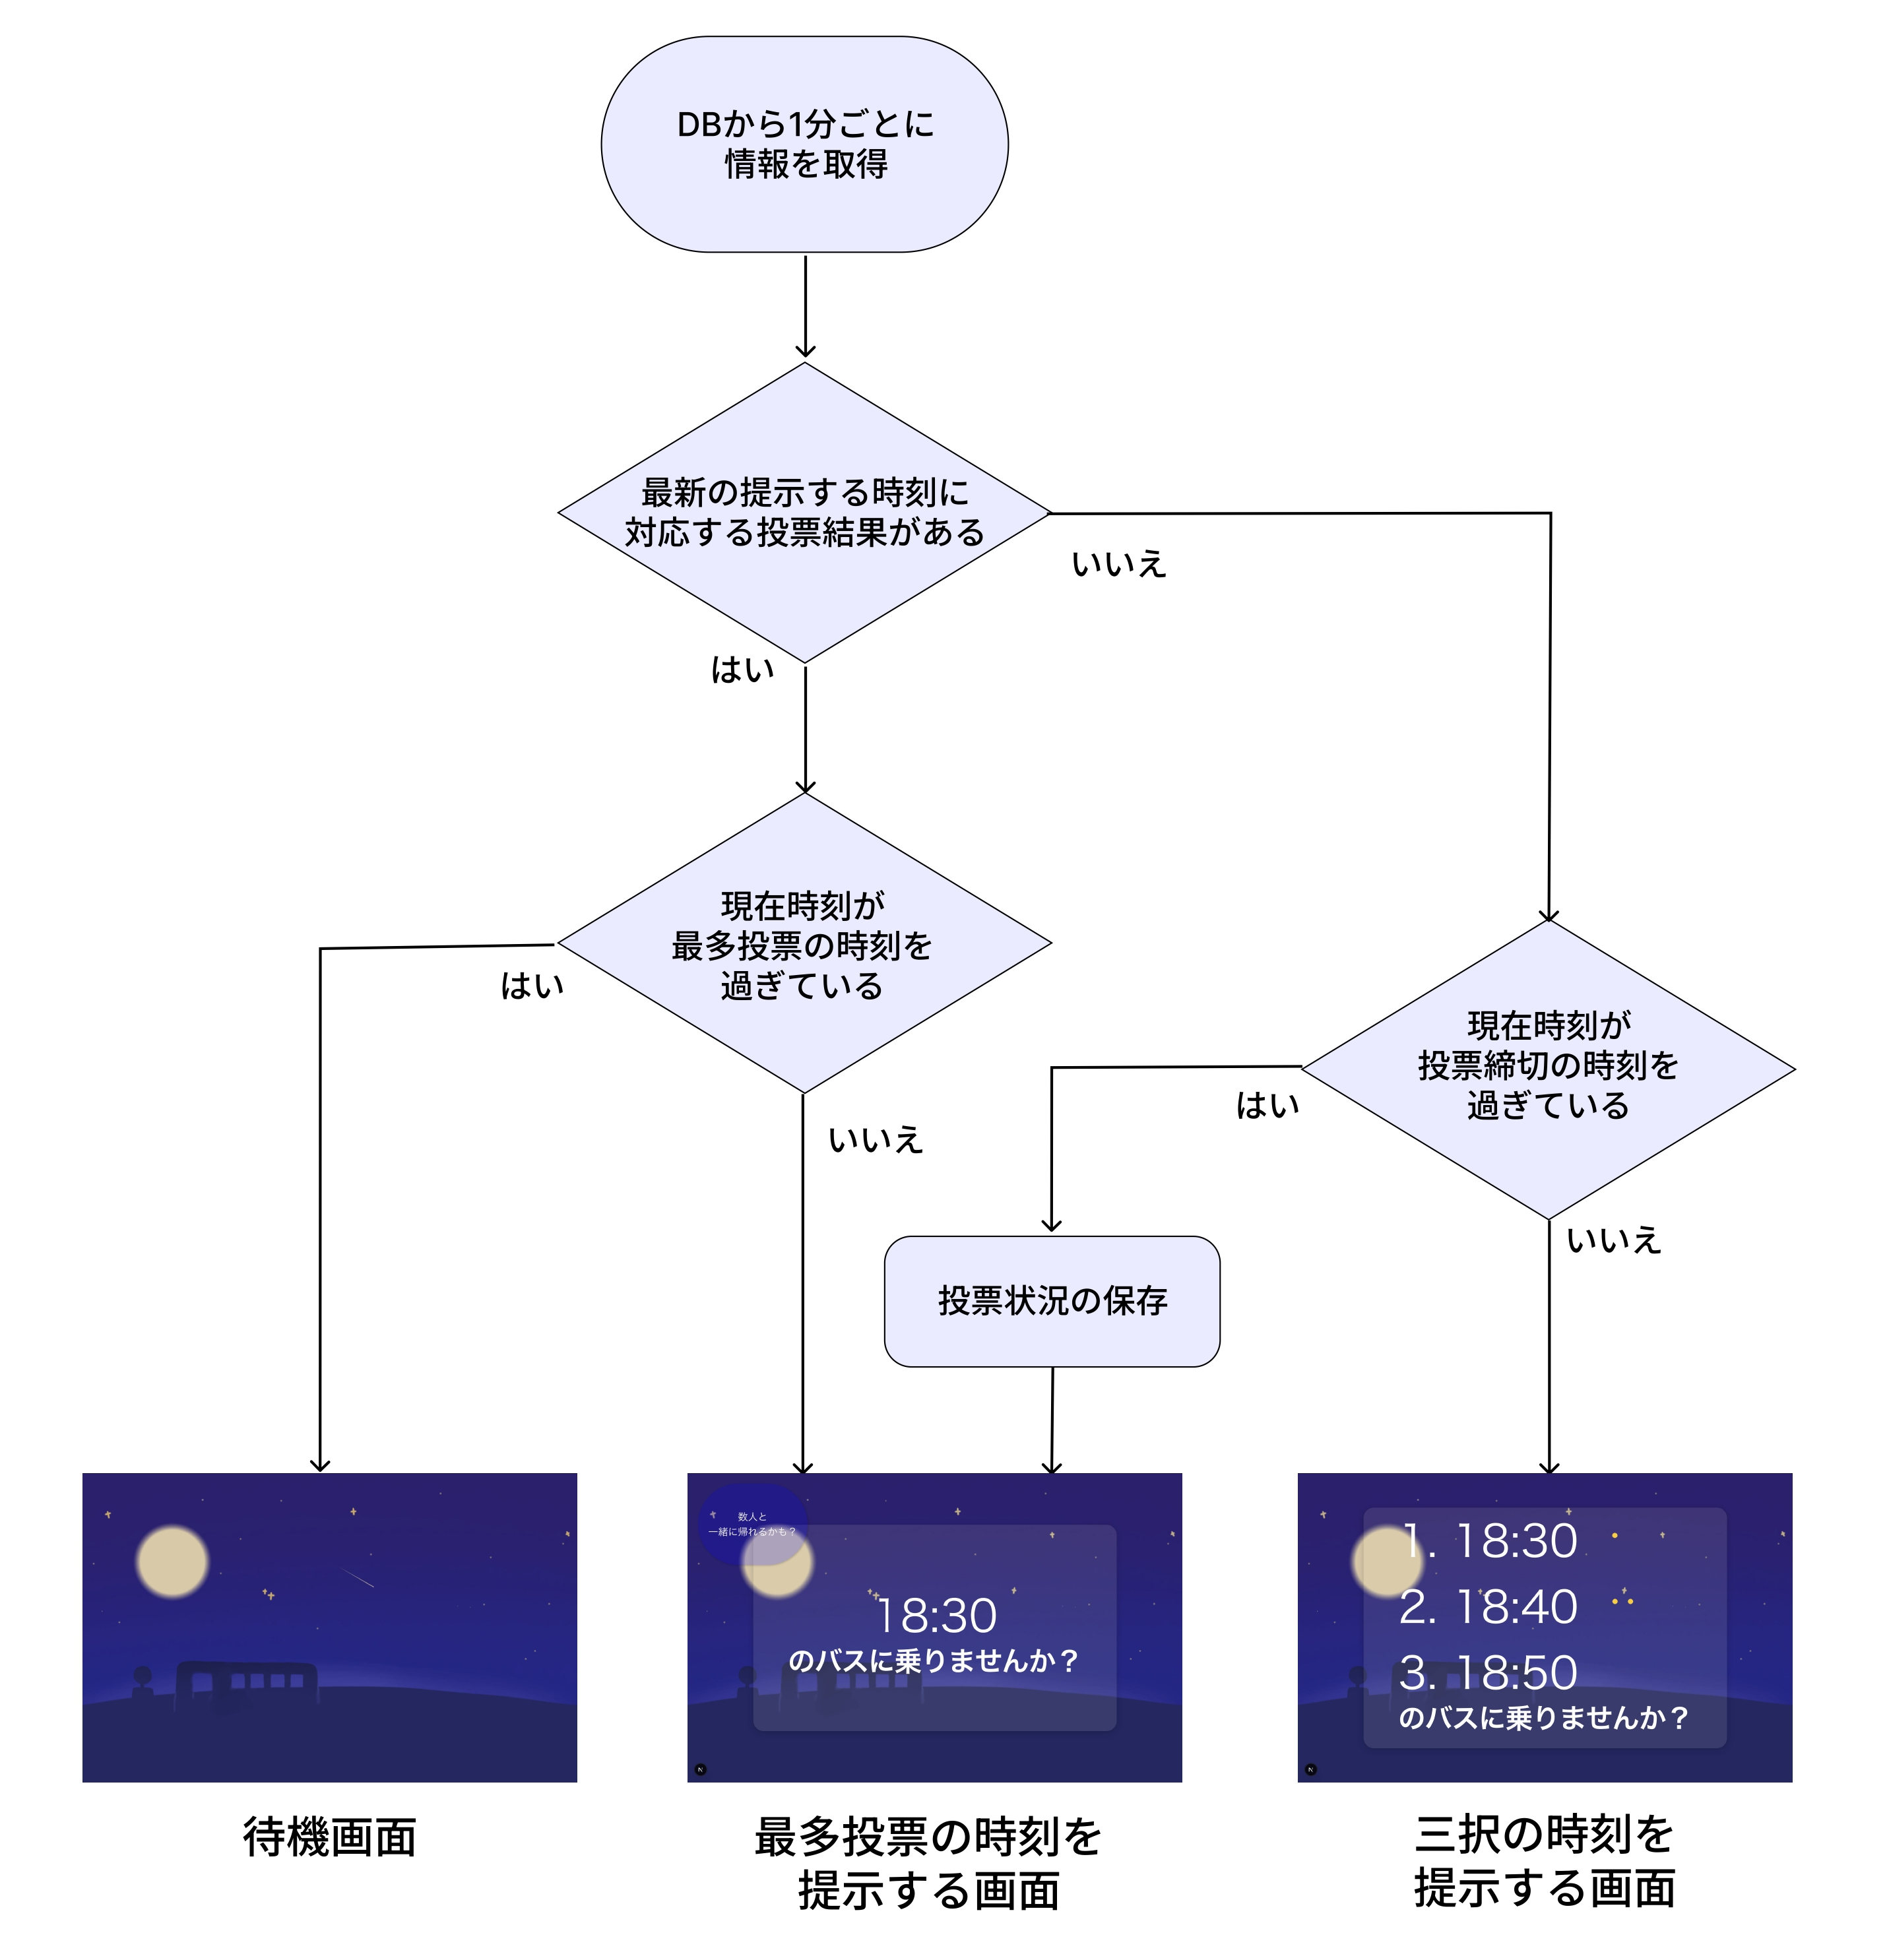
\includegraphics[width=0.9\linewidth]{fig/flow.jpg} % suzuki
  \caption{画面遷移}
  \label{fig:disflow}

\end{figure}

\subsection{三択の時刻を提示する画面}
この画面では三択の時刻と，それぞれの時刻への投票数を表示する．
実際の画面を図\ref{fig:selectDisplay}に示す．
この画面への遷移時には音声による通知を行い，画面表示の変化に気づきやすくしている．
また，投票状況を時刻横に丸の数として反映し，他の人の投票を参考に帰宅時刻の検討や変更ができる設計としている．
現在時刻が投票締切時刻をすぎた際に最多投票の時刻を提示する画面へと自動的に遷移する．

\begin{figure}[htb]
  \centering
  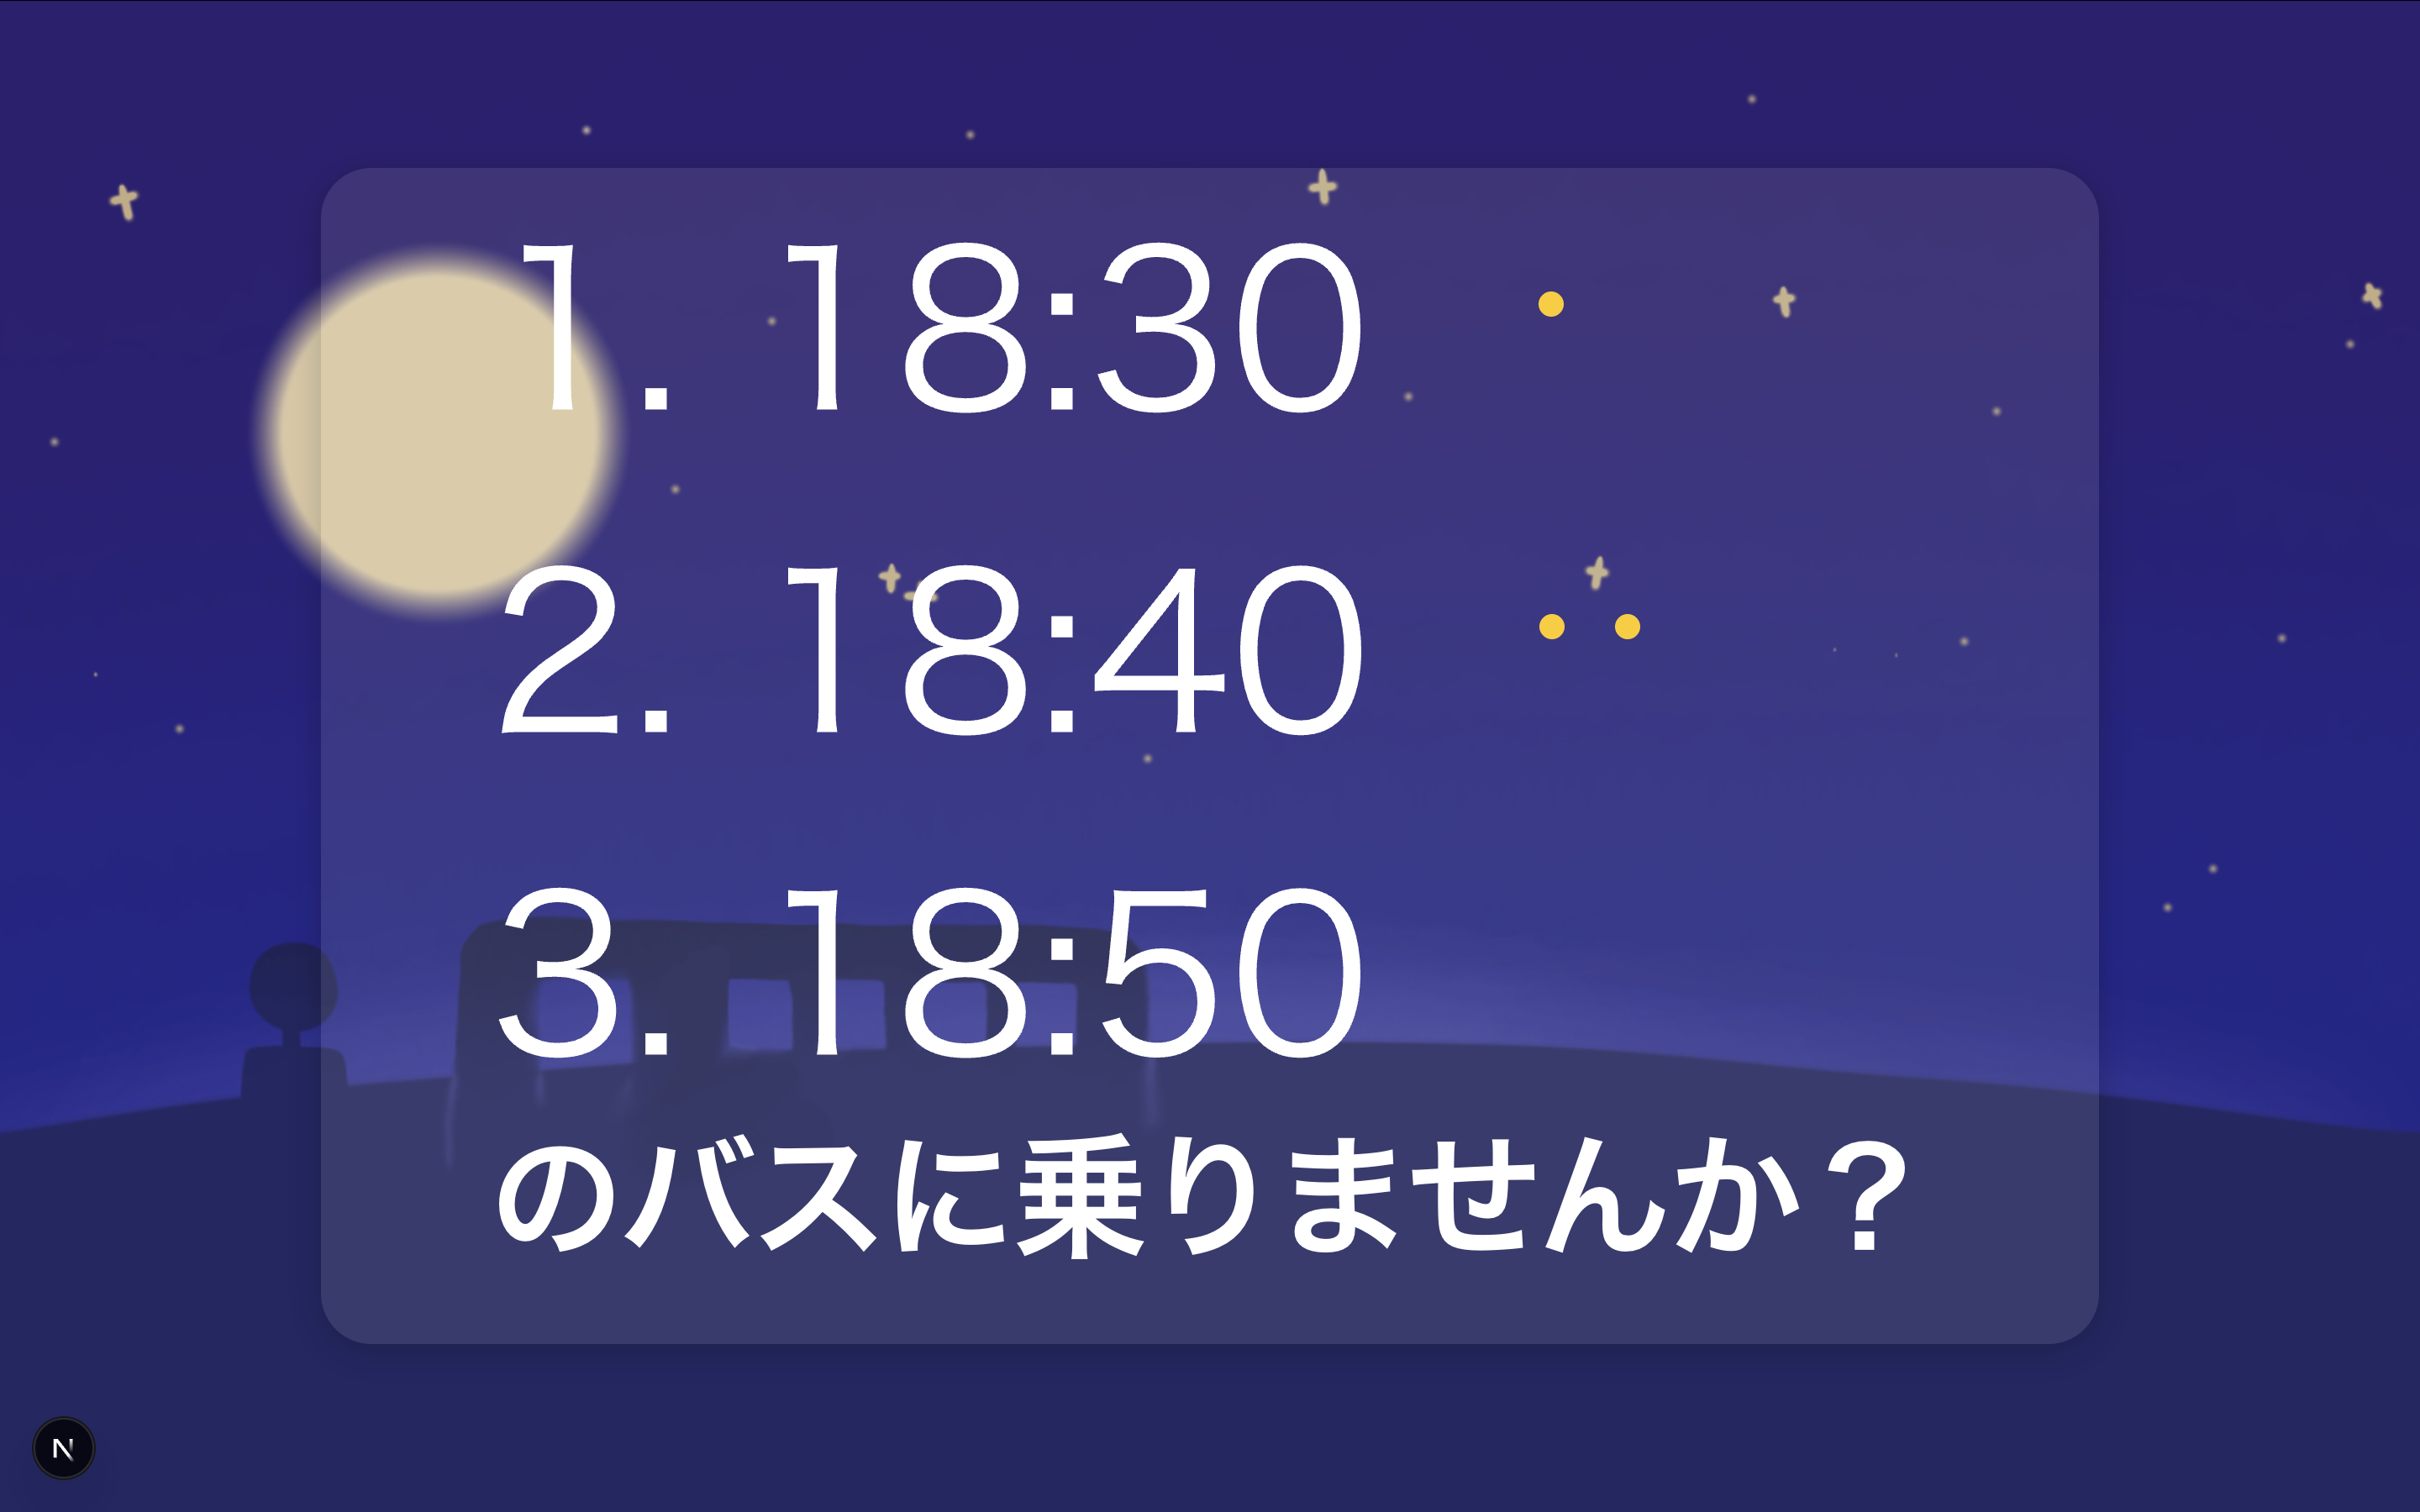
\includegraphics[width=0.7\linewidth]{selectDisplay.png} % suzuki
  \caption{三択の時刻を提示する画面}
  \label{fig:selectDisplay}

\end{figure}

本画面の設計にあたっては，設置環境や利用状況を踏まえた視認性および理解のしやすさに配慮した．
本画面は，共有スペースに設置された小型のモニターでの利用も想定し，離れた位置からでも内容を把握できるよう，時刻情報を画面内で大きく表示する設計とした．
また，各選択肢には数字を対応させ，ユーザが直感的に投票操作を行えるようにした．
加えて，「〜のバスに乗りませんか？」という表現を用いて，提示している時刻とバスの出発時刻の対応を一目で理解できるよう工夫した．
各時刻への投票状況は具体的な人数を数値で表示するのではなく，点の数として視覚的に表現した．
これにより，他者の選択傾向を直感的に把握できる一方で，人数の多寡を過度に強調せず，選択に対する心理的な圧力を和らげる意図がある．

また，本システムでは画面遷移への気づきを促すための一手段として音声通知を併用した．
通知に用いる音声には読み上げソフトである音読さん\cite{ondoku}を利用して作成した．
具体的には，「おすすめのバスの時刻が設定されました」という短い文言を読み上げた音声を用い，三択の提示画面へ遷移するタイミングで再生する．
音声内容は，ユーザに対して新たな情報提示が行われた事実のみを簡潔に伝える設計とし，周囲で行われている既存の対面コミュニケーションを過度に遮らないよう配慮した．
音声は画面遷移への気づきを促す目的で用い，具体的な時刻情報は表示画面に集約する設計とした．

この音声通知の作成にあたっては，画面遷移への気づきを促しつつも，通知時間が過度に長くならないよう配慮した．
具体的には，読み上げ音声の再生速度を標準よりやや速い設定とし，短時間で内容を伝えられるよう調整した．
また，周囲の環境音の中でも認識されやすいよう，比較的高めの声色を選択して音声を作成した．
以上のように，本システムにおける音声通知は，画面表示を中心とした情報提示を補完する手段として位置付けている．
\subsection{最多投票の時刻を提示する画面}

この画面では投票数が最も多かった時刻とその投票数を表示する．
実際の画面を図\ref{fig:resultDisplay}に示す．
この画面への遷移時に投票数の集計および表示を行う．
投票結果に基づき，最も帰宅行動につながりやすいと考えられる時刻を選択して表示する．
また，投票人数の表示方法を工夫し，声かけを行う際の心理的負担を軽減する設計とした．
現在時刻が表示している時刻をすぎた際に待機画面へと自動的に遷移する．
\begin{figure}[htb]
  \centering
  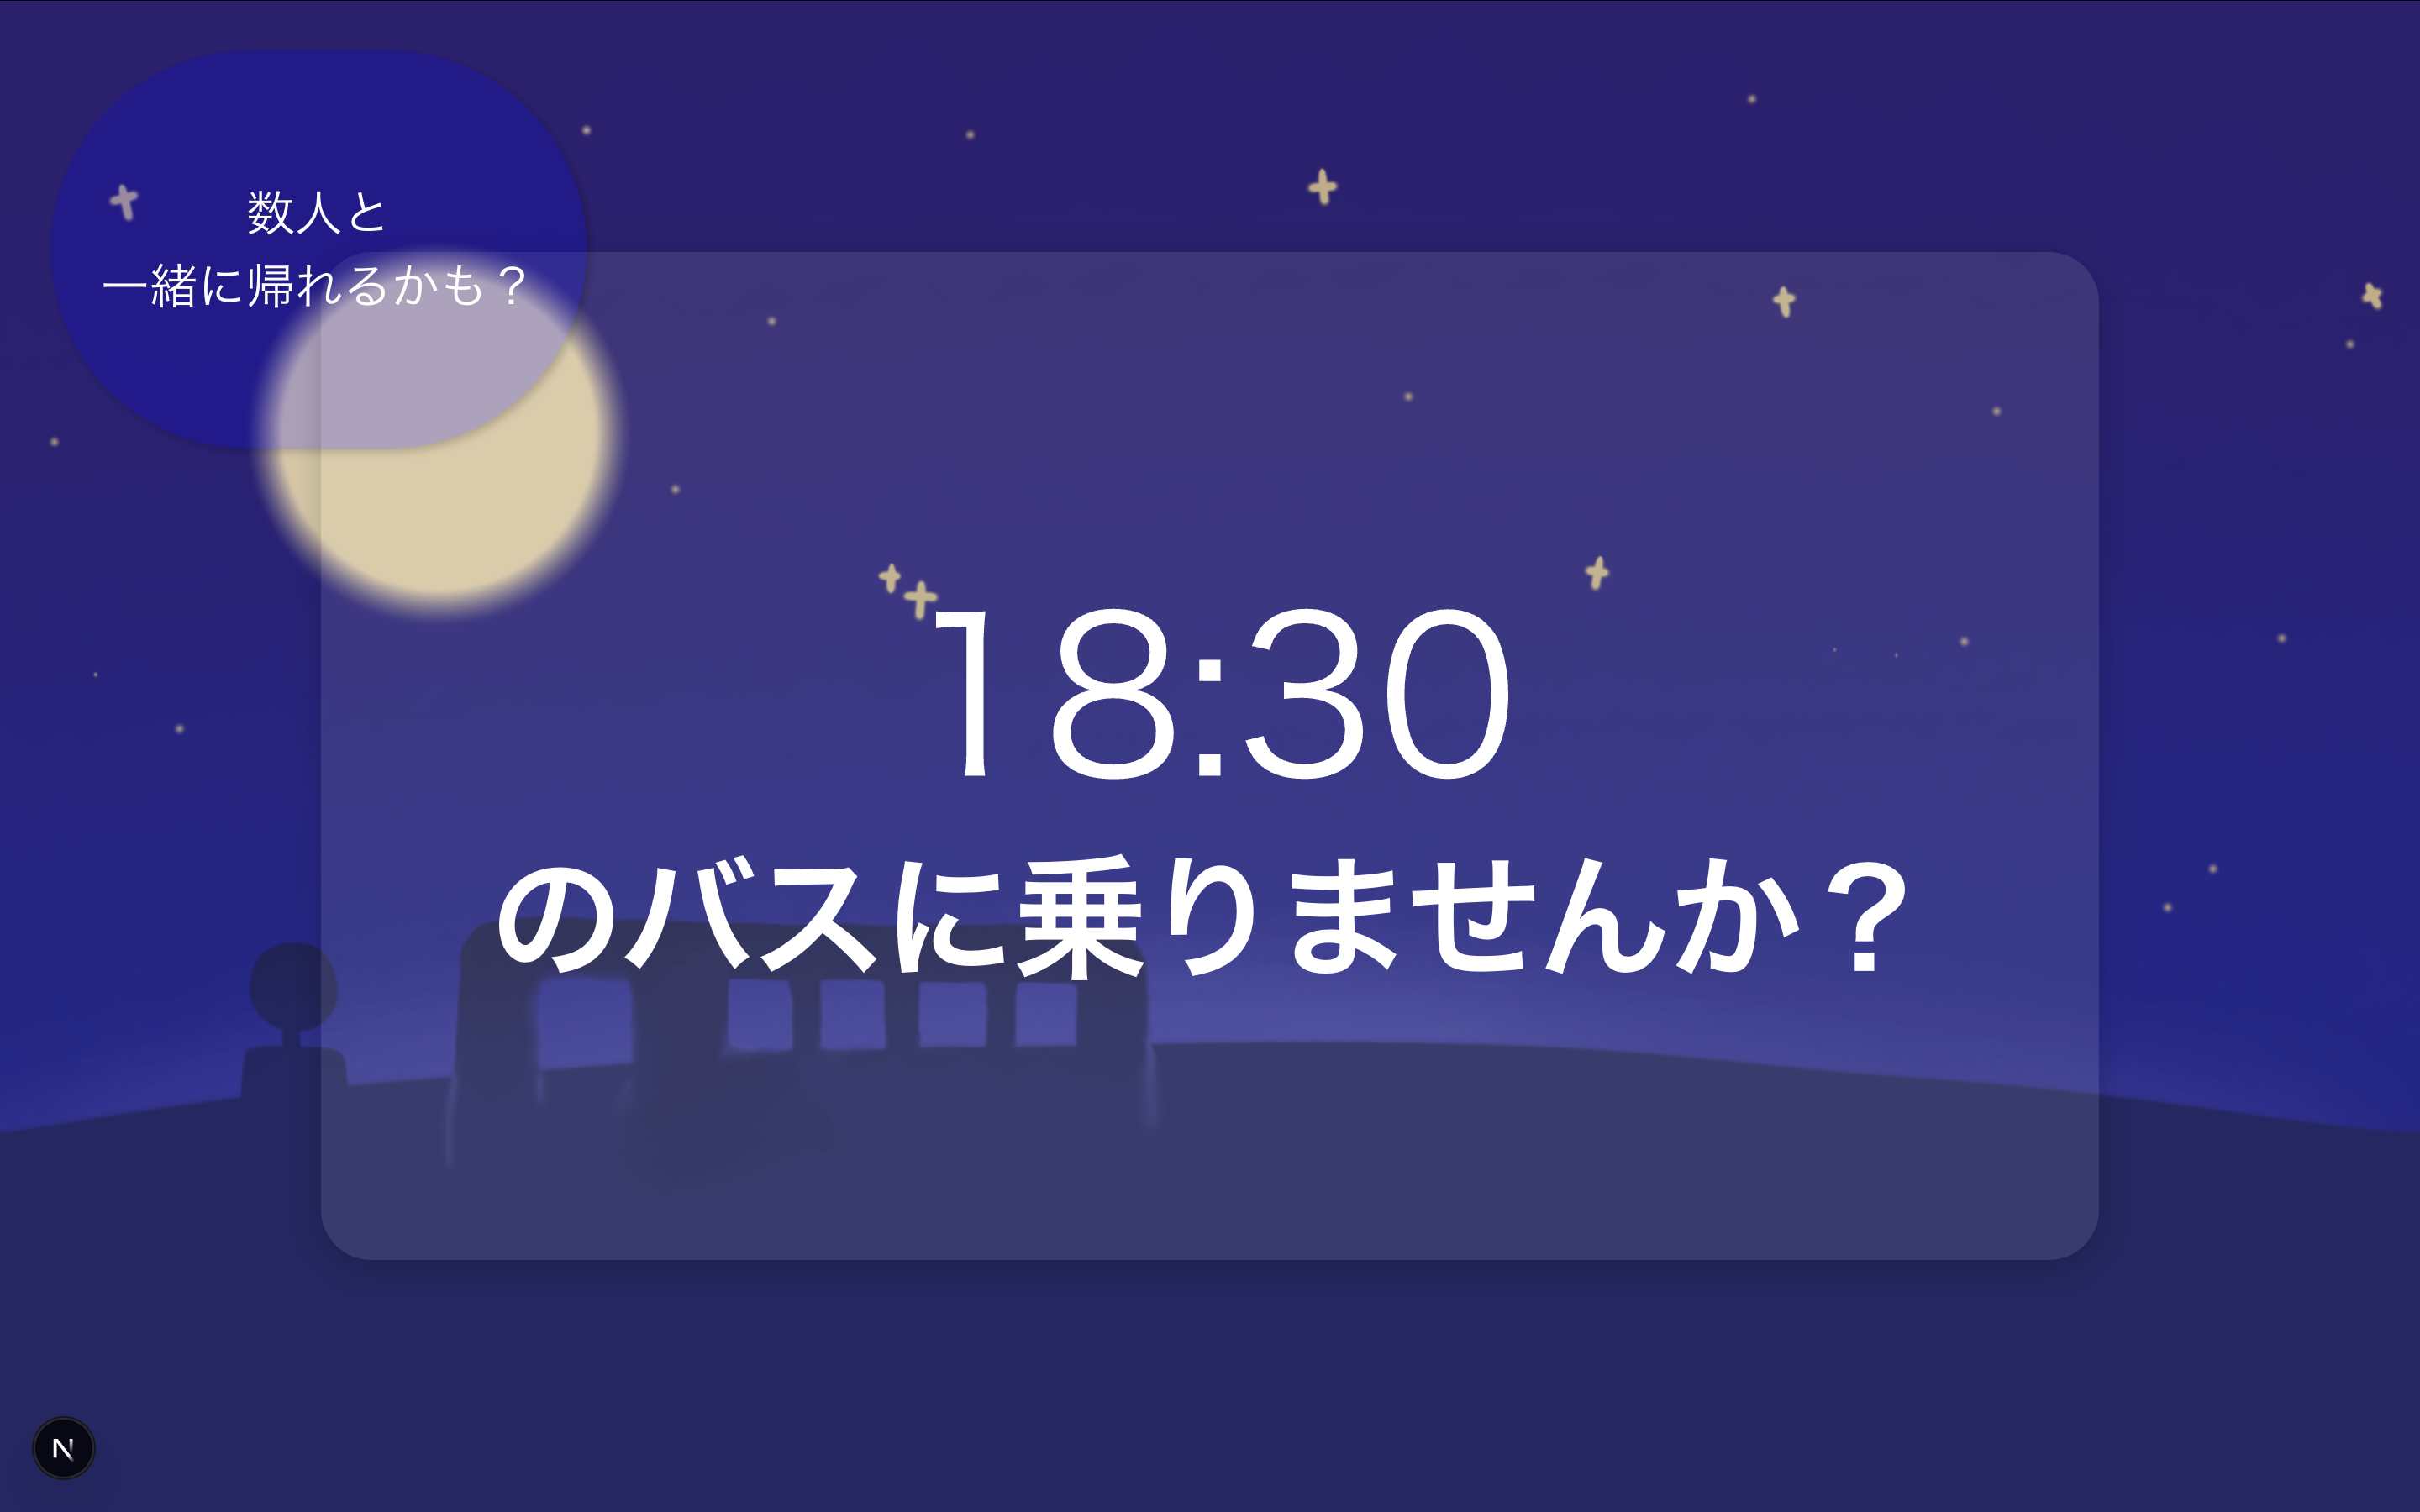
\includegraphics[width=0.7\linewidth]{resultDisplay.png} % suzuki
  \caption{最多投票の時刻を提示する画面}
  \label{fig:resultDisplay}

\end{figure}

% 本画面においても，離れた位置から内容を把握できるよう，帰宅時刻を画面内で大きく表示する設計とした．
% 本画面は，三択の投票結果をもとに，利用者の帰宅行動を一つの時刻へ収束させることを目的としている．
% 投票数が最も多かった時刻を強調して提示し，その時刻に帰宅可能な利用者が比較的多いと視覚的に示す設計とした．
% また，投票がなかった場合には，最も帰りやすいと考えられる帰宅推奨時刻に近い時刻を表示する．
% 同票の時刻が存在する場合には，各時刻の帰宅同行が成立する可能性が同程度であると判断し，より多くの利用者が帰宅行動を起こす前の時刻として，早い時刻を選択する．
% 一方で，投票人数に関する情報は，画面に近づいた際に確認できる程度の大きさとした．
% これにより，帰宅意思を持つ利用者が詳細情報を確認しやすくなる一方で，周囲にいる他の利用者に対して過度な情報提示とならないよう配慮している．
本画面においても，離れた位置から内容を把握できるよう，帰宅時刻を画面内で大きく表示する設計とした．
また，投票数が最も多かった時刻を強調して提示し，三択の投票結果の中で帰宅可能なユーザが比較的多い時刻を視覚的に示す．
一方で，投票人数に関する情報は，画面に近づいた際に確認できる程度の大きさとした．

本画面は，三択の投票結果をもとに，ユーザが帰宅しやすい時刻を一つに絞り込む目的で設計している．
したがって，投票がなかった場合には最も帰宅しやすいと考えられる帰宅推奨時刻に近い時刻を選択する．
同票の時刻が存在する場合には，各時刻の帰宅同行が成立する可能性が同程度であると判断し，より多くのユーザが帰宅行動を起こす前の時刻として，早い時刻を選択する．
また，投票人数の表示方法についても，声かけを行う際の心理的負担を抑える観点から設計している．

なお，本システムでは「おすすめの退室時刻」ではなく，利用者が目標とする行動の基準として「乗車すべきバスの時刻」を提示している．
これは，「この時刻までに出れば余裕をもって間に合う時刻」と「実際に出発すれば間に合う最終的な時刻」との間に存在する時間帯において，何も情報が提示されない状態を避けるためである．
また，この時間帯のみ表示内容や画面構成を切り替えると，利用者にとって表示規則が分かりにくくなる可能性がある．
そのため，本画面では一貫してバスの時刻を基準とした提示に専念し，実際に建物を出る時刻の判断は利用者に委ねる設計とした．


投票人数の表示方法については，人数の多寡によって表現を切り替えている(図\ref{fig:resultDisplays})．
具体的には，無投票の場合は人数表示を行わず，1票の場合には「数人と一緒に帰れるかも？」という抽象的な表現を用いた．
2票以上の場合には「〜人と一緒に帰れるかも？」と具体的な人数を示す．
これは，投票したユーザがその時刻に帰宅可能であると仮定し，「一緒に帰れる可能性」を提示し，声かけを行う際の心理的なハードルを下げる意図で設計した．

\begin{figure}[htb]
  \centering
  \subcaptionbox{無投票の場合}{
    
\includegraphics[width=0.3\linewidth]{0.png}}	% suzuki
  \hspace{3mm}
  \subcaptionbox{投票数が1の場合}{
    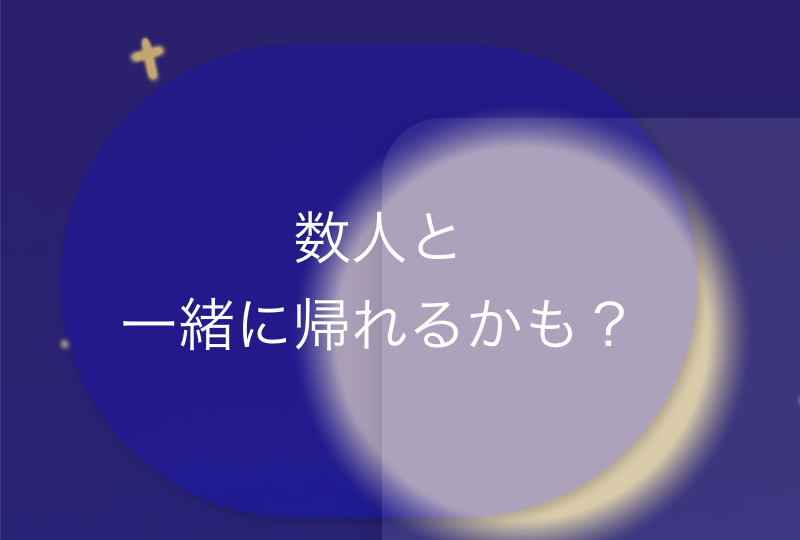
\includegraphics[width=0.3\linewidth]{1.png}}	% suzuki 
  \hspace{3mm}
  \subcaptionbox{投票数が複数の場合}{
    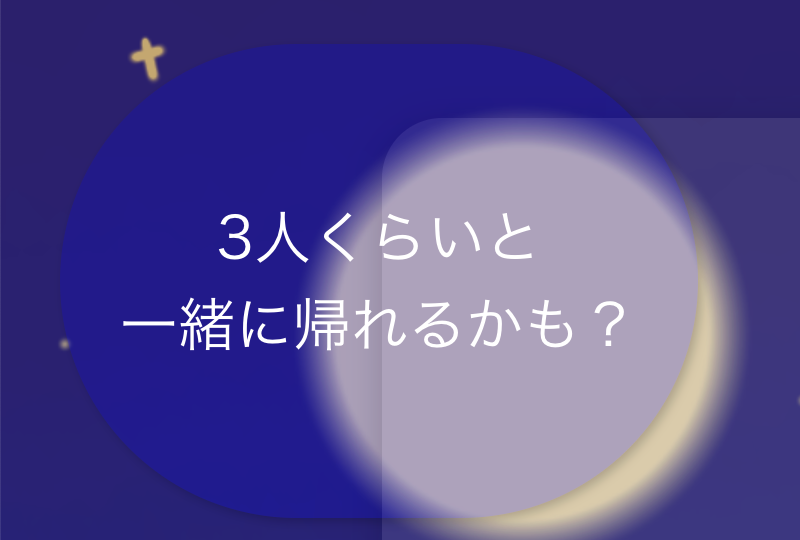
\includegraphics[width=0.3\linewidth]{3.png}}
  \caption{投票人数の提示箇所}
  \label{fig:resultDisplays}
\end{figure}
\subsection{待機画面}

% 以上の2つの画面でない状況を示す．
本画面は，三択の時刻を提示する画面および最多投票の時刻を提示する画面のいずれにも該当しない状態を明確に示すための画面である．
投票対象外の時間帯や，投票が開始される条件を満たしていない場合，および表示された投票結果の時刻を過ぎた場合に図\ref{fig:waitingDisplay}(\subref{fig:wait})のように表示される．
新たに三択の時刻が設定された際に三択の時刻を提示する画面へと自動的に遷移する．

また，システムが稼働中であると示すため，画面内に小さな動きを付与している．
これは，画面が停止していると誤認されるのを防ぎ，ユーザに対してシステムが正常に動作していると伝える意図がある．

さらに，投票対象外の時間帯であると視覚的に示すため，図\ref{fig:waitingDisplay}(\subref{fig:stop})のように画面全体を暗く表示している．
対象外の時間帯は，一般的に深夜および早朝とされる22:00から6:59までとし，この時間帯においては帰宅同行を促す情報提示を抑制する設計とした．

\begin{figure}[htb]
  \centering
  \subcaptionbox{条件外の場合の画面\label{fig:wait}}{
    
\includegraphics[width=0.4\linewidth]{fig/waitingDisplay.png}}	% suzuki
  \hspace{3mm}
  \subcaptionbox{対象外の時間の画面\label{fig:stop}}{
    
\includegraphics[width=0.4\linewidth]{fig/stoppingDisplay.png}}	% suzuki 
  \caption{待機画面}
  \label{fig:waitingDisplay}
\end{figure}

% \begin{figure}[htb]
%   \centering
%   \subcaptionbox{三択の時刻}{% % suzuki
%     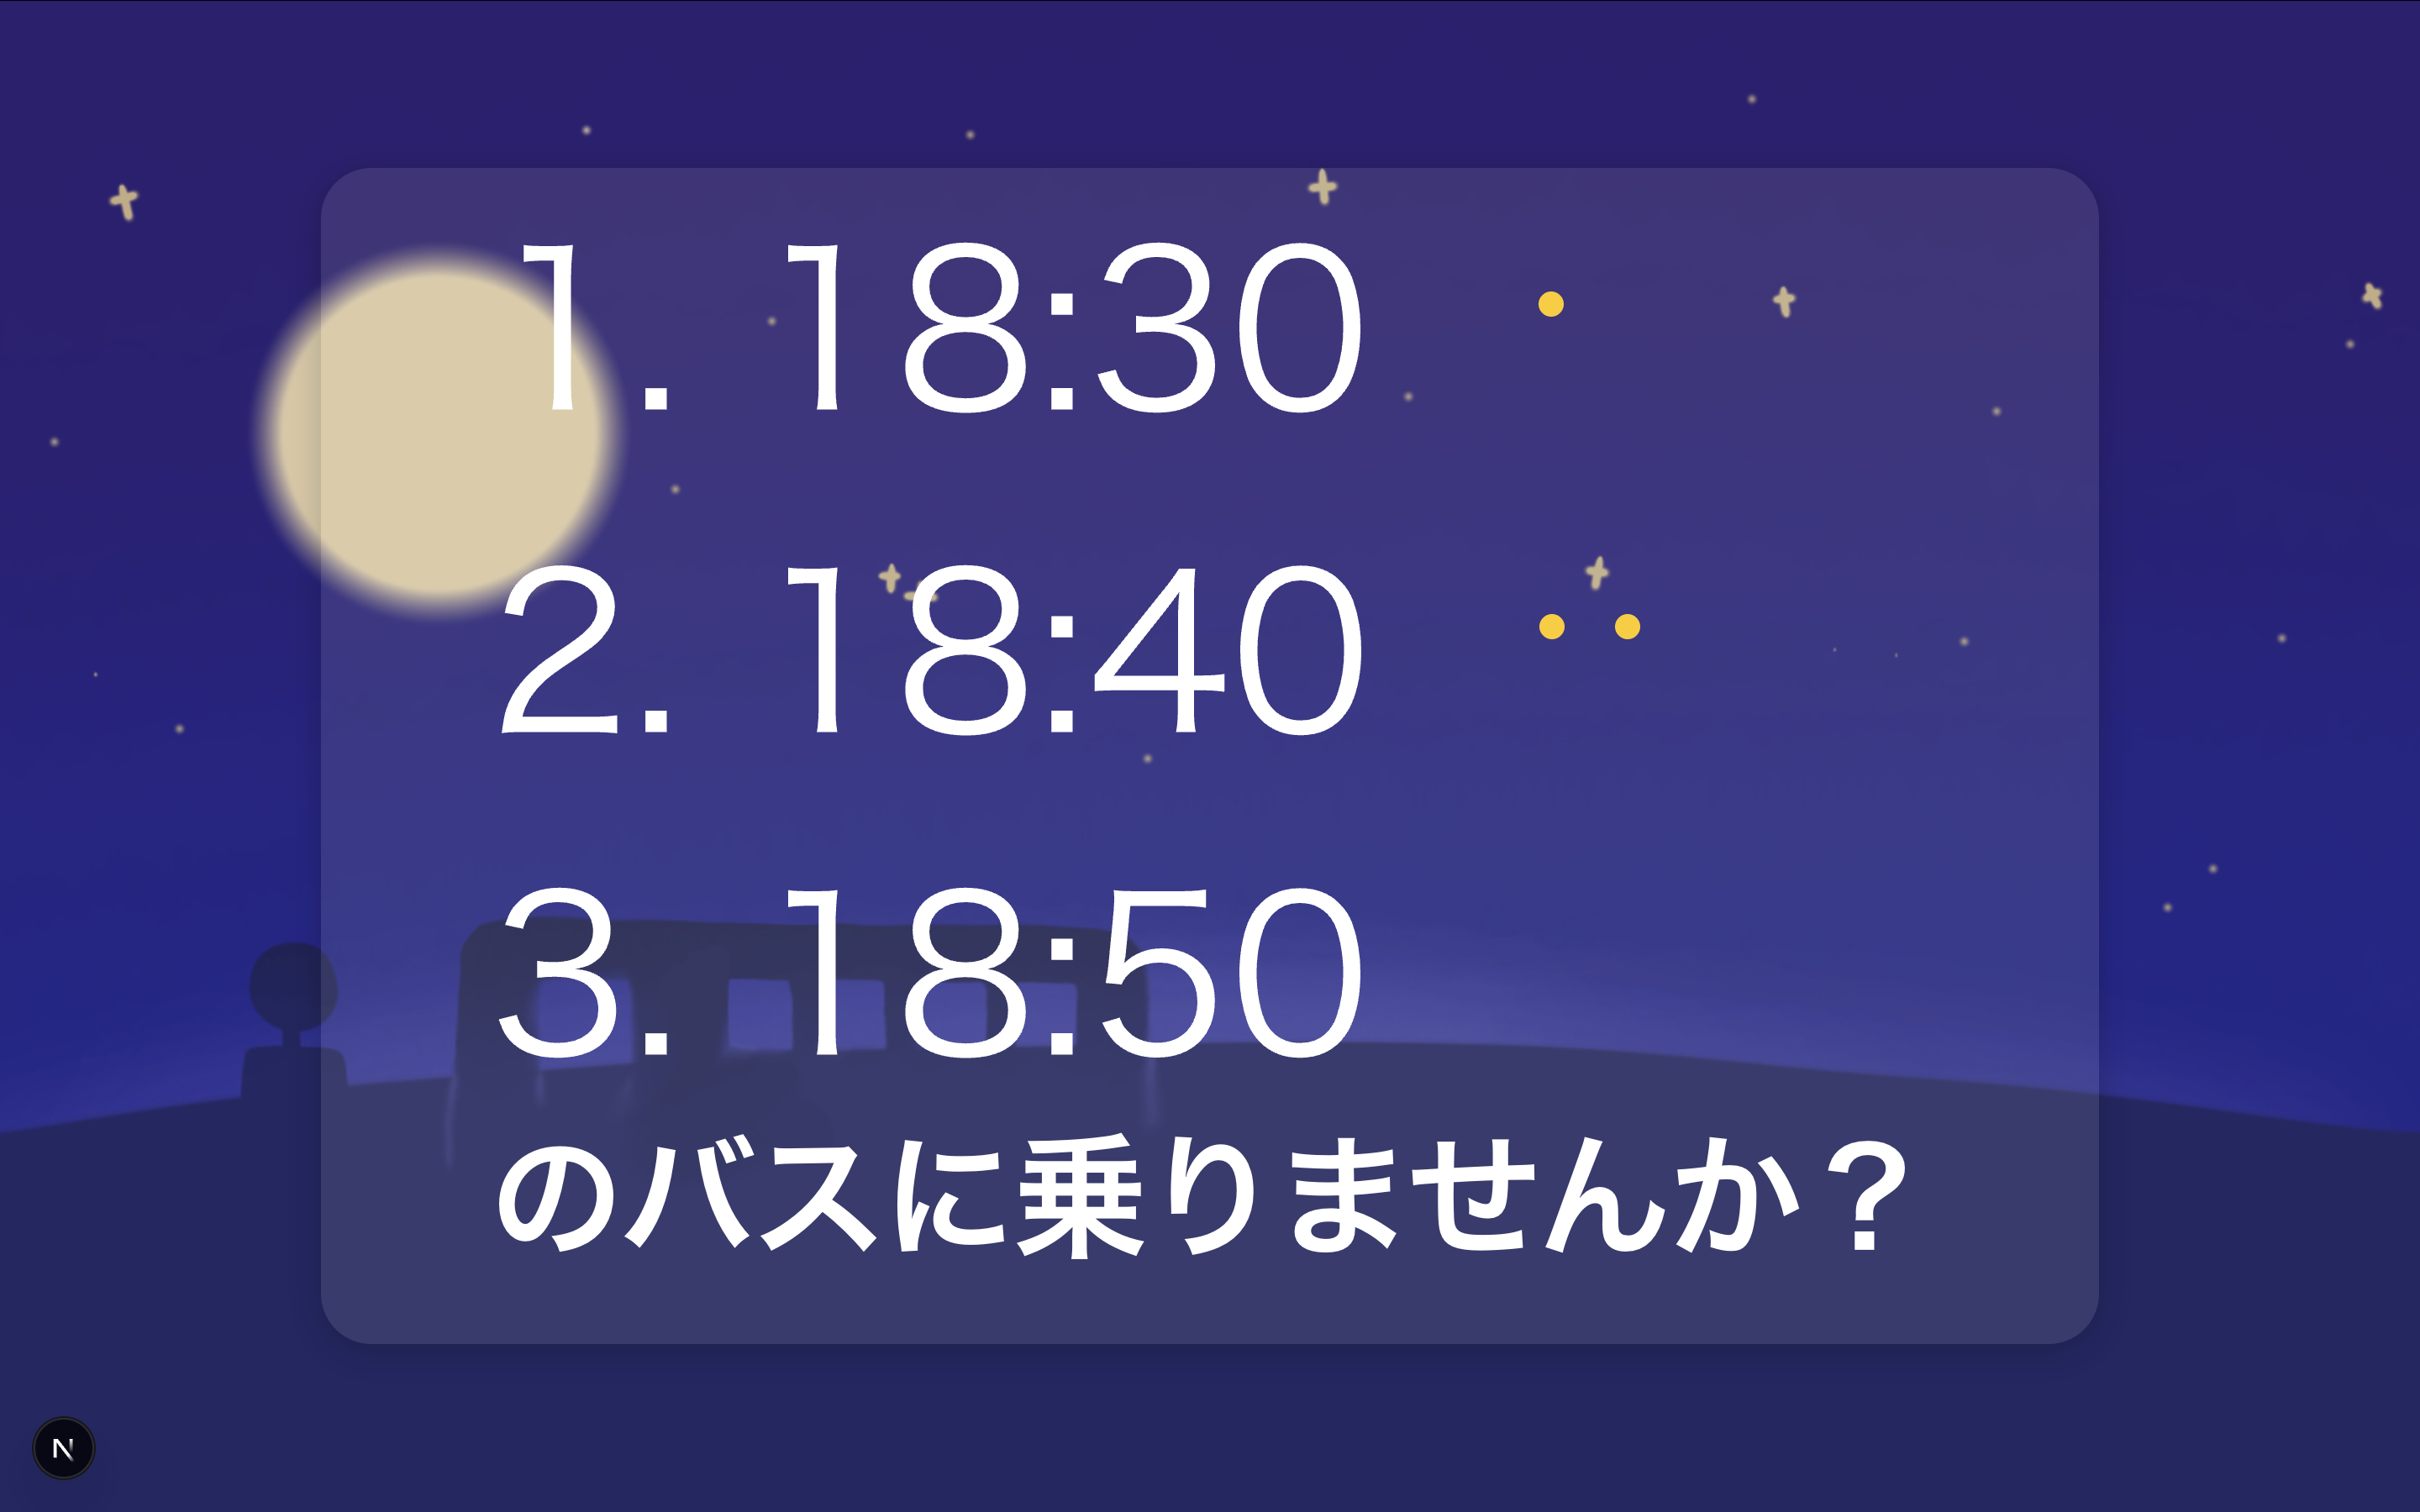
\includegraphics[width=0.4\linewidth]{selectDisplay.png}}	% suzuki
%   \hspace{3mm}
%   \subcaptionbox{最多投票の時刻}{%	% 良く考えたら投票人数による表示の違い全部載せた方がいいのでは？
%     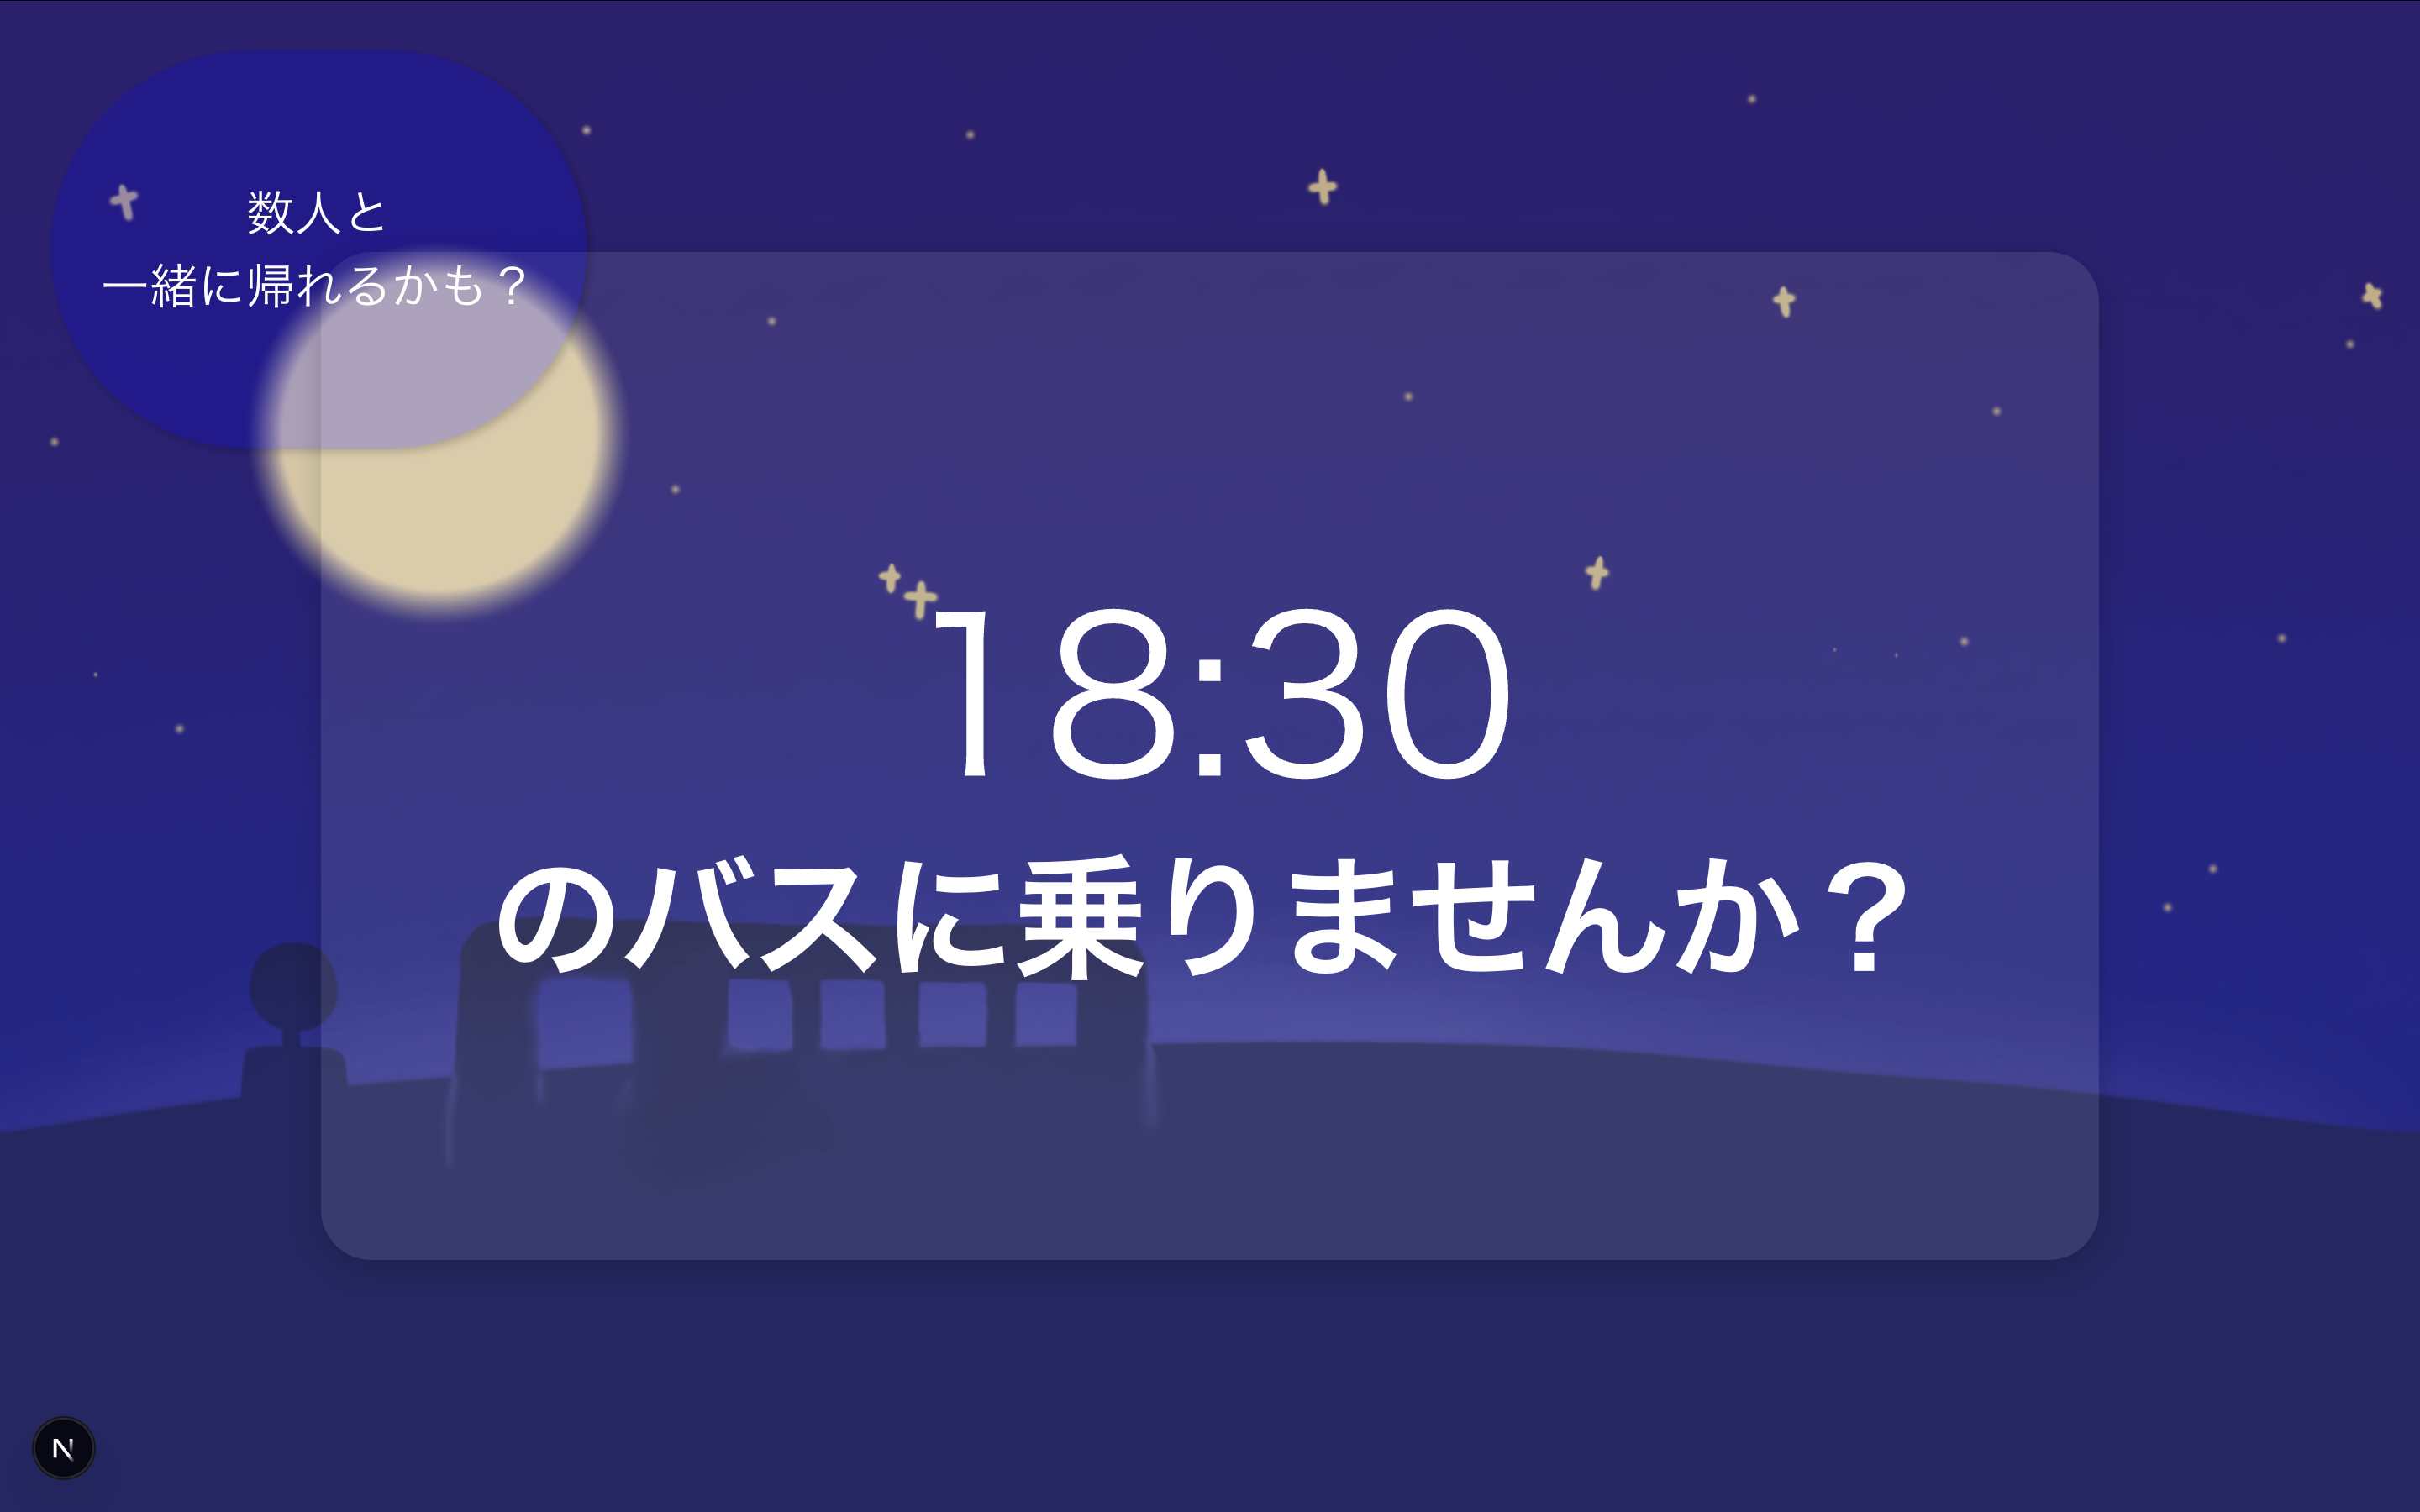
\includegraphics[width=0.4\linewidth]{resultDisplay.png}}	% suzuki 
%   \caption{時刻の提示を行う画面}
%   \label{fig:2}
% \end{figure}
